\documentclass{article}

% Language setting
% Replace `english' with e.g. `spanish' to change the document language
\usepackage[french]{babel}
\usepackage[fleqn]{amsmath} % Aligner les équations à gauche


% Set page size and margins
% Replace `letterpaper' with`a4paper' for UK/EU standard size
\usepackage[letterpaper,top=2cm,bottom=2cm,left=3cm,right=3cm,marginparwidth=1.75cm]{geometry}

% Useful packages

\usepackage{amsmath}
\usepackage{graphicx}
\usepackage{subcaption}
\usepackage[colorlinks=true, allcolors=blue]{hyperref}

\title{TD 7 - Sujets d'électrostatique}
\author{IPESUP - PC }
\date{06/11/23}

\begin{document}
\maketitle

\section{Energie d'une boule}

Calculer l'énergie d'une boule de rayon $R$ et uniformément chargée de charge $\rho$. \\
Bonus: Pareillement, calculer la puissance du laser de l'étoile de la mort.

\section{CCINP 2021}

Questions 1 à 9. 

\section{Mines 2022 Sujet 2}

Questions 1, 2 et 5 à 9. \\[2cm]

\begin{figure}[h]
    \centering
    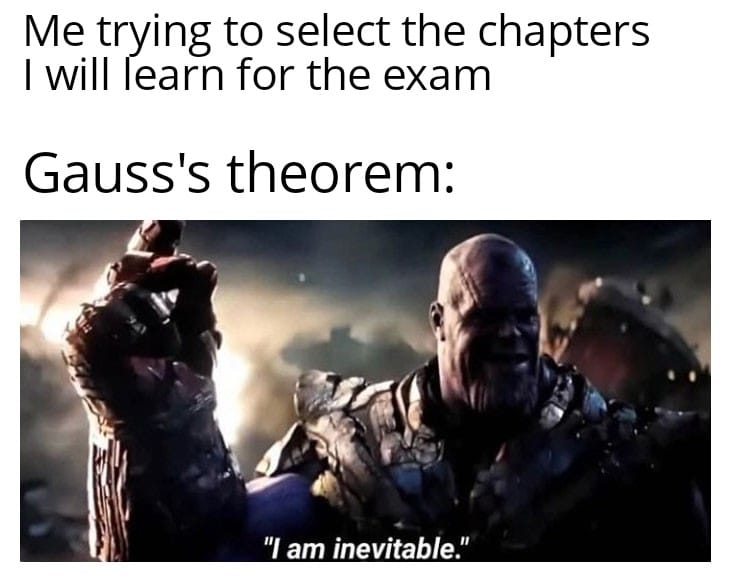
\includegraphics[width=0.55\textwidth]{meme.jpg}
\end{figure}

\end{document}

